\documentclass{scrartcl}
\usepackage[misc]{ifsym}
\usepackage[utf8]{inputenc}
\usepackage[T1]{fontenc}
\usepackage{ctex}
\usepackage{xspace}
\usepackage{enumerate}
\usepackage{colonequals}
\usepackage{stmaryrd}
\usepackage{todonotes}
\usepackage{amsmath,amscd,amsbsy,amssymb,latexsym,url,bm,amsthm}
\usepackage{epsfig,graphicx,subfigure}
\usepackage{hyperref}
\usepackage{xcolor}
\usepackage{tikz}
\usepackage{appendix}
\usepackage[vlined,ruled,commentsnumbered,linesnumbered]{algorithm2e}
\usepackage{enumerate,fullpage,proof}
% style adjustments

\renewcommand{\arraystretch}{1.5}

% References

\bibliographystyle{plainurl}
\newcommand{\sref}[1]{{\tiny[#1]}}

% general stuff
\newcommand{\stackl}[2]{\vtop{\hbox{\strut#1}\hbox{\strut#2}}}
\newcommand{\stackc}[2]{\vtop{\setbox0\hbox{\strut #1}\copy0\hbox to\wd0{\hss\strut #2\hss}}}
\newcommand{\stackr}[2]{\vtop{\setbox0\hbox{\strut #1}\copy0\hbox to\wd0{\hss\strut #2}}}

% remember TikZ positions.
\newcommand{\tmark}[1]{
  \tikz[remember picture, baseline, inner xsep=0, inner ysep=0.2em]{ \node [anchor=base] (#1) {\vphantom{M}};
}}%

% listings

\usepackage{listings}

\newcommand*{\lstitem}[1]{
  \setbox0\hbox{\lstinline{#1}}  
  \item[\usebox0]  
  % \item[\hbox{\lstinline{#1}}]
  \hfill \\
}

\newcommand{\lst}{\lstinline}
\lstdefinelanguage{Coq}%
  {morekeywords={Variable,Inductive,CoInductive,Fixpoint,CoFixpoint,%
      Definition,Lemma,Theorem,Axiom,Goal,Local,Save,Grammar,Syntax,Intro,%
      Trivial,Qed,Intros,Symmetry,Simpl,Rewrite,Apply,Elim,Assumption,%
      Left,Cut,Case,Auto,Unfold,Exact,Right,Hypothesis,Pattern,Destruct,%
      Constructor,Defined,Fix,Record,Proof,Induction,Hints,Exists,let,in,%
      Parameter,Split,Red,Reflexivity,Transitivity,if,then,else,Opaque,%
      Transparent,Inversion,Absurd,Generalize,Mutual,Cases,of,end,Analyze,%
      AutoRewrite,Functional,Scheme,params,Refine,using,Discriminate,Try,%
      Require,Load,Import,Scope,Open,Section,End,match,with,Ltac,%
      Instance,Class,%
      bind,as,%
	},%
   sensitive, %
   morecomment=[n]{(*}{*)},%
   morestring=[d]",%
   literate={=>}{{$\Rightarrow$}}1 {>->}{{$\rightarrowtail$}}2{->}{{$\rightarrow$}}1
   {forallx}{{$\forall\!\!$}}1
   %{>>}{\scomp}1
   %{<>}{{$\neq$}}1 indeed... no.
  }[keywords,comments,strings]%

\lstset{
   basicstyle=\ttfamily,
   keywordstyle=\bfseries\color{blue}
  }
\lstset{language=Coq}
\lstset{columns=fullflexible, keepspaces}
\usetikzlibrary{arrows,shapes,chains}
\newtheorem{thm}{Theorem}

\begin{document}
\title{An online search engine for classical Chinese poems}
\author{Xiwei Wu \& Ning Yang \& Hui Ma}

\date{}
\maketitle

\begin{abstract}
  \textbf{Abstract:} This is a group-based project for Web Search \& Mining. In this project, we implemented a poetry crawler that crawled more than 10,000 poems from https://www.shi-ci.com/ from pre-Qin to modern times, then implemented a search engine that can support a variety of different search requirements, and finally provided a web front-end that can be easily used. 

\textbf{Keywords: Scrapy, Chinese poems, search engine}
\end{abstract}

\section{Introduction} \label{sec:intro}







\noindent \textbf{Outline.} In Section \ref{sec:crawl}, we will introduce our crawler based on Scrapy and SQL. In Section \ref{sec:search}, we will introduce our design for search engine. In Section \ref{sec:web}, we will introduce our design for web front-end. In Section \ref{sec:concl}, we will give a demonstration of the results of our project.
# Automatically created by: scrapy startproject
#
# For more information about the [deploy] section see:
# https://scrapyd.readthedocs.io/en/latest/deploy.html

[settings]
default = poems.settings

[deploy]
#url = http://localhost:6800/
project = poems

\section{Search Engine} \label{sec:search}

We use Python to build the entire search engine, and a series of data structures, such as DataFrame are used to build our entire search engine.

\subsection{Overall Design}

The entire search process is as follows: first, based on the SQL database, we built several dictionaries and stored the entire SQL database into a DATAframe \lstinline{df_all}, along with the rank information we decided. After a series of processes, our engine initialization is complete and enter the query phase.

After asking user to get the query type and query content, we process the content according to the query type, and then make the corresponding query within \lstinline{df_all}, return the results for output, and ask the user whether to continue the query. We will describe how to implement these steps in the following sections.

All the codes are in\textbf{ 'process.py'} and \textbf{'run.py'}. You can use Python run \textbf{run.py} to start this system.

\subsection{Data Process}

First, after reading into the database, we stored it in the DataFrame \lstinline{df_all} for easy processing, and the attributes are as previously mentioned : dynasty, poet name, poem name, contents, poet description. Also, for subsequent zone-specific queries, we store two dictionaries of poem name and contents.

Then, for Boolean search, we construct a term dictionary. And consider the complexity of the grammar of Chinese ancient poetry, we decide to think a single word as a term. According to this idea, we construct the term dictionary \lstinline{dict_word}. Based on the dictionary, we process and obtain a 0-1 vector for each ancient poem and construct the term-poem incidence matrix, and the matrix is  \lstinline{matrix_binary_all}. In each vector, 1 means the word  appears in the poem corresponding to this position and 0 means not.

Finally, we appended two sets of ranking values to each ancient poem according to the ranking we thought about and added them to \lstinline{df_all}. The entire data processing process is completed.


\subsection{Boolean Search}

The user input a string include search keys and operations, 
for each search key, we convert it to a 0-1 vector based on the dict we got before. For multiple single words inside the search key, we get all the corresponding vectors and then do \lstinline{AND} on them. Then we check each result we get to make sure that the search key is actually present in the result, not scattered throughout the poem. 

Then for each search key, we perform the corresponding \lstinline{AND, OR, NOT} operation, and get the final result vector. And, unlike the documentation requirements,  we have included dynasties and authors in the search


And finally, all search methods, including this one, will end up with a vector, and then the \lstinline{vec_to_outlist} and  \lstinline{outlist_to_out} functions will be called to output the corresponding poems. This step is not repeated in the following search.

Here are three examples of searches.


\begin{figure*}[h]
\centering
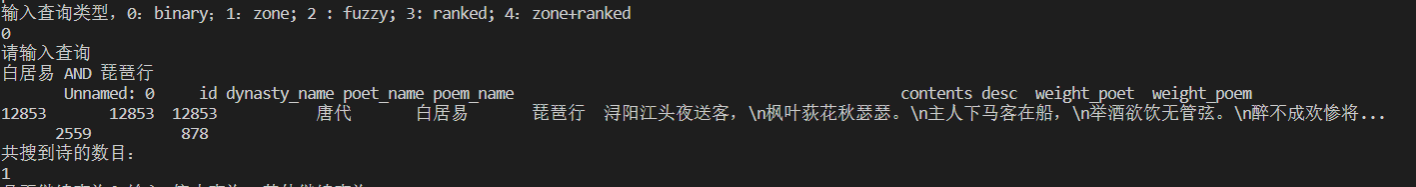
\includegraphics[width=0.8\textwidth]{figure/boolean-1.png}
\caption{Boolean Search example 1: search with AND. We search '白居易 AND 琵琶行', and return 1 result, which is correct.}
\label{search-1}
\end{figure*}

\begin{figure*}[h]
\centering
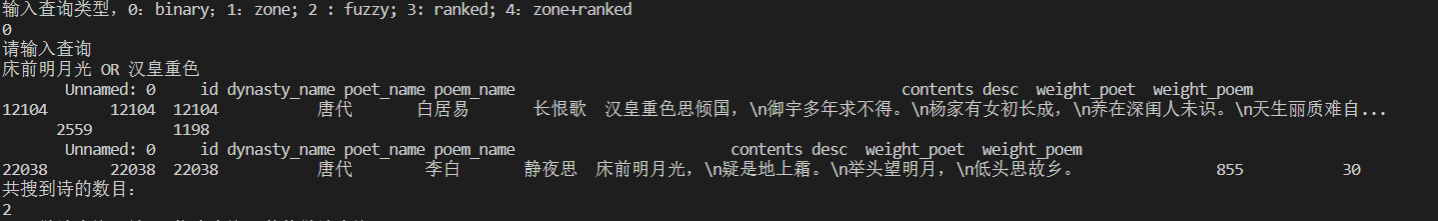
\includegraphics[width=0.8\textwidth]{figure/boolean-or.png}
\caption{Boolean Search example 2: search with OR. We search '床前明月光 OR 汉皇重色', and return 1 result, which is correct.}
\label{search-2}
\end{figure*}

\begin{figure*}[h]
\centering
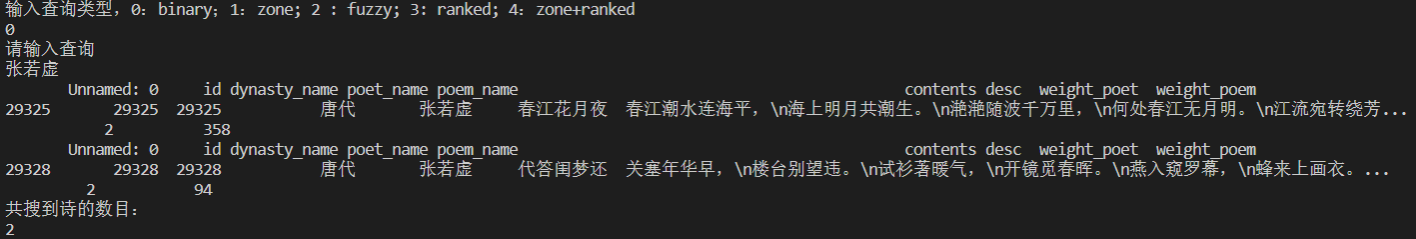
\includegraphics[width=0.8\textwidth]{figure/not-1.png}
\label{search-3}
\end{figure*}

\begin{figure*}[h]
\centering
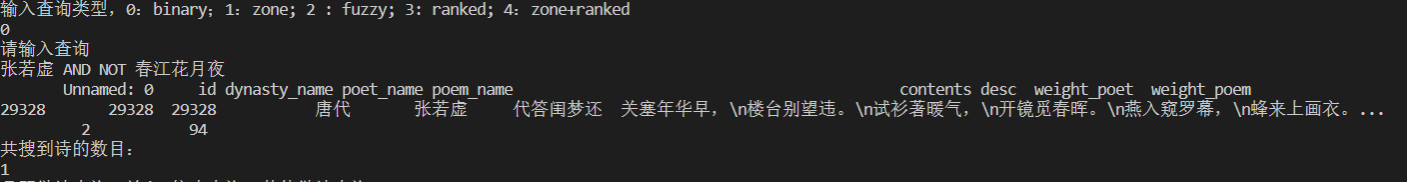
\includegraphics[width=0.8\textwidth]{figure/not-2.png}
\caption{Boolean Search example 3: search with NOT. We search '张若虚', and return 2 result; if we search '张若虚 NOT 春江花月夜', and we will get 1 result, the specified item is excluded from the search results. }
\label{search-4}
\end{figure*}


\subsection{Zone-specific Search}

The dynasty, author,title and content are entered in order, or keep empty. For enumerable attributes like author and dynasty, the returned vector only contain those exactly match the query, where we use the query function of DataFrame, 

\begin{lstlisting}
    list = df_all.loc[df_all.dynasty_name == dynasty]
    list = df_all.id[df_all.poet_name == author]
\end{lstlisting}

And we use Boolean search on title and content. At last, we do \lstinline{AND} on the four returned vectors to get the final out, empty set as all-1 vector.

The example is shown in fig\ref{search-5} and fig\ref{search-6}.

\begin{figure*}[h]
\centering
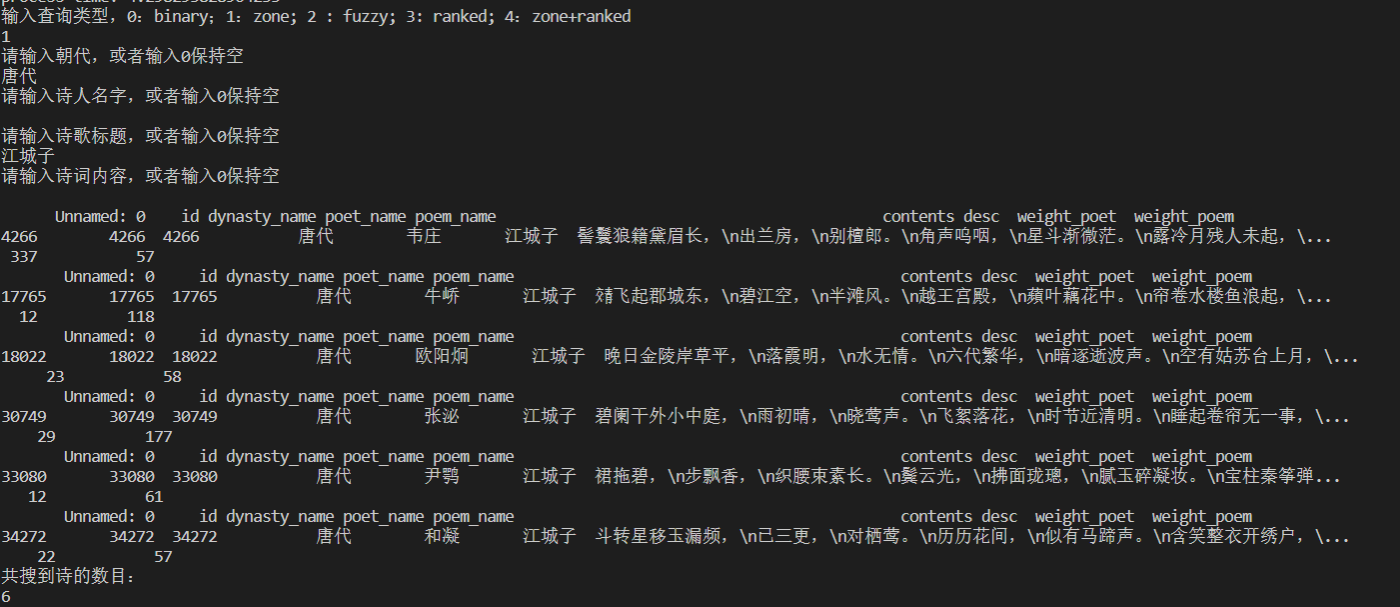
\includegraphics[width=0.7\textwidth]{figure/zone-1.png}
\caption{Zone-specific Search example 1: We search '江城子' as title and '唐代' as dynasty, and return 6 results, all meet the requirements.}
\label{search-5}
\end{figure*}

\begin{figure*}[h]
\centering
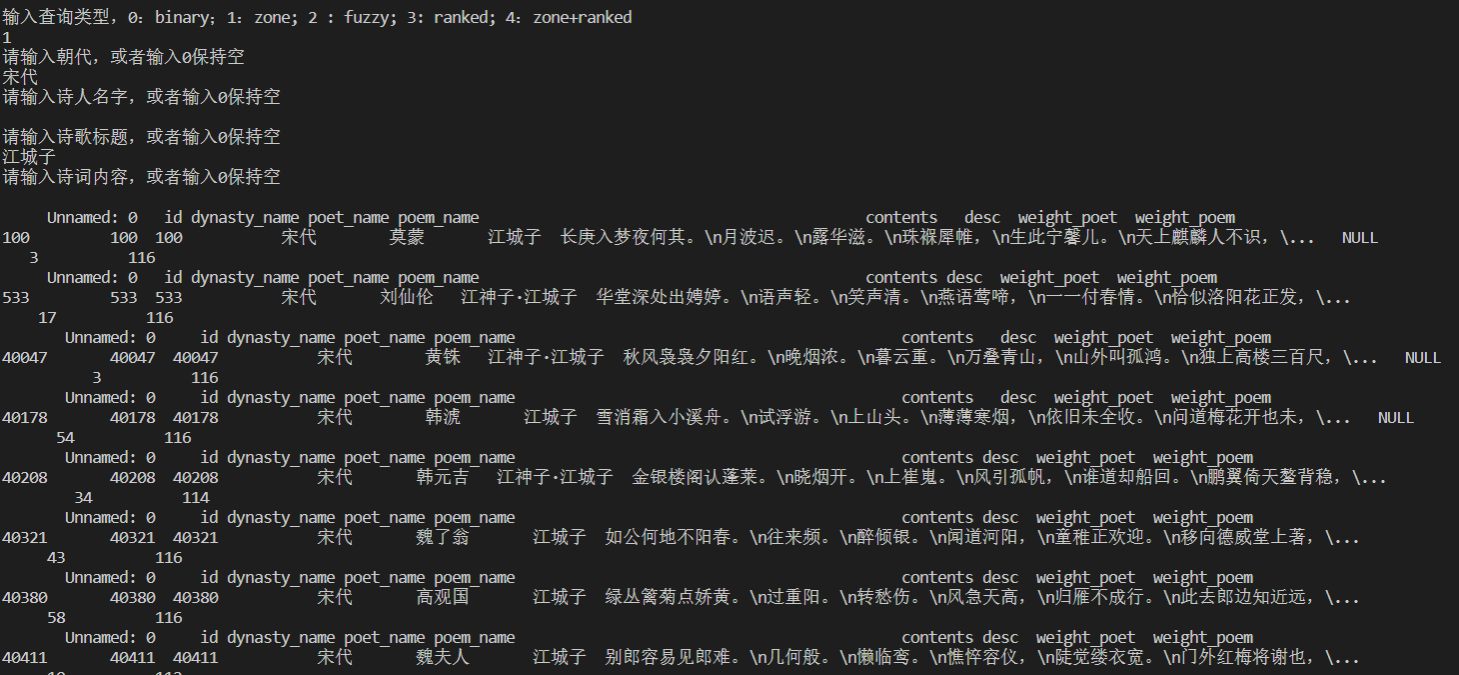
\includegraphics[width=0.7\textwidth]{figure/zone-2-103.png}
\caption{Zone-specific Search example 2: We search '江城子' as title and '宋代' as dynasty, and we can see that there are 103 results, and all meet the requirements.}
\label{search-6}
\end{figure*}



\subsection{Pinyin-based Tolerant Search}

To handle the fuzzy search based on pinyin, we created a table of Chinese characters to pinyin correspondence, which can be found in poem/data/pinyin.txt. For every word of the target to be searched, we will do single word substitution according to the pinyin, and  do a Boolean search, then connect each different returned vector with \lstinline{OR}.

Finally, we use \lstinline{AND} to link all the single word vectors and output.

Such a search has several advantages and several disadvantages, the advantages of such search method is very powerful, as long as the pin-yin is right, it will definitely return the correct result, but there are corresponding cost. The number of results returned may be large, and the search time may be longer, there is no guarantee that the results the user wants will be at the top of the list. It may be possible to optimize further with a fuzzy search rank, but the search will take longer. Taking all things into account, we decided to keep this search the way it is now.

The example is shown in fig\ref{search-7}.


\begin{figure*}[h]
\centering
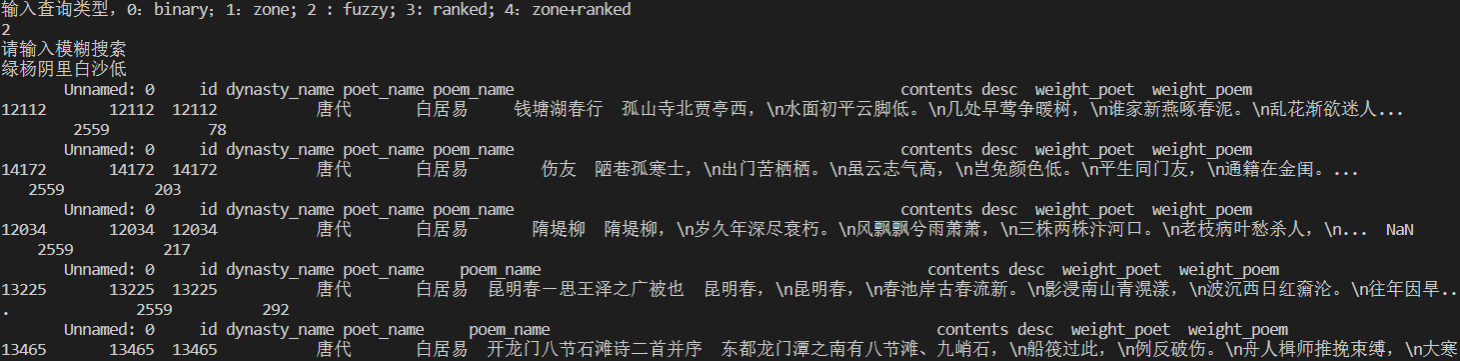
\includegraphics[width=0.8\textwidth]{figure/fuzzy-example.png}
\caption{Fuzzy Search example: We search '绿杨阴里白沙低' , with correct '堤' is changed to the homophonic '低', and we can see that expected correct result is returned.}
\label{search-7}
\end{figure*}

\subsection{Ranked Search}

First, the search result is based on Boolean search, but here we no longer support logical operations. We have thought and discussed, and have come up with some ranking bases. One caveat is that poetry ordering is very subjective and varies from person, so we do not guarantee that our ordering will be the best in all cases. Here are some thoughts:

Intuitively, for the same content, it appears at the beginning or at the end, we usually prefer the former;

For the same content, if it appears in the poet, the title, the dynasty and the content of the poem, we want the poet is the first appears in the results, the title second, and the dynasty and the content.

For the fame of the poet, since there is no necessarily correct measure method, we used a more intuitive measure: the  more poems this poet had, the more likely he was famous. For those poets who are very famous but have few works now, this may not be the right standard, but for most poets, this is the right standard.

And, for users, they always prefer short content to lengthy content, so we will put shorter poems in front.

Based on these idea, we measured each poem the number of  poems retained by the author and the length of the poem, and add them to \lstinline{df_all}. This process is very time-consuming(about 2-3 minutes), so we store the \lstinline{df_all} as a csv so that we don't have to wait too long after one initialization.

Before the final output, we use \lstinline{query_seq} to do these rank, first we sort the poems according to content's length, then we sort the poems in reverse order according to the the number of poems retained by the author, at last we sort the poems according to location where the query appears.

The more the author's work and the shorter the poem, the earlier the query is matched, the more this result will be in front. 

For the other queries, since the query is composite, we only sorted the poem length and the number of poems, and the function is \lstinline{query_seq_noquery}.

By the way, because of the presence of a large number of anonymous poets(“无名氏”), in order to ensure that they do not unduly affect the ranking of normal poets we manually weighted their number of poems to 1.


The example is shown in \ref{search-8}, we use same key to get different result return order.


\begin{figure*}[h]
\centering
\subfigure[1]{
\begin{minipage}{0.8\linewidth}
\centering
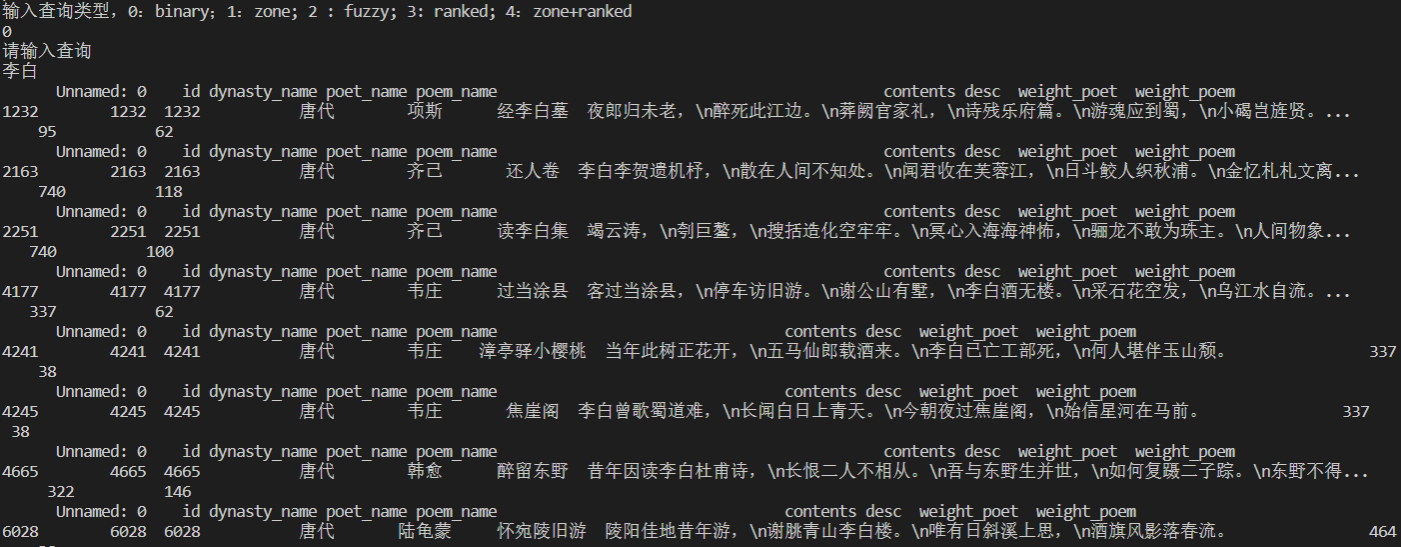
\includegraphics[width=0.8\textwidth]{figure/rank-1.png}
\end{minipage}
}

\subfigure[2]
{
\begin{minipage}{0.8\linewidth}
\centering
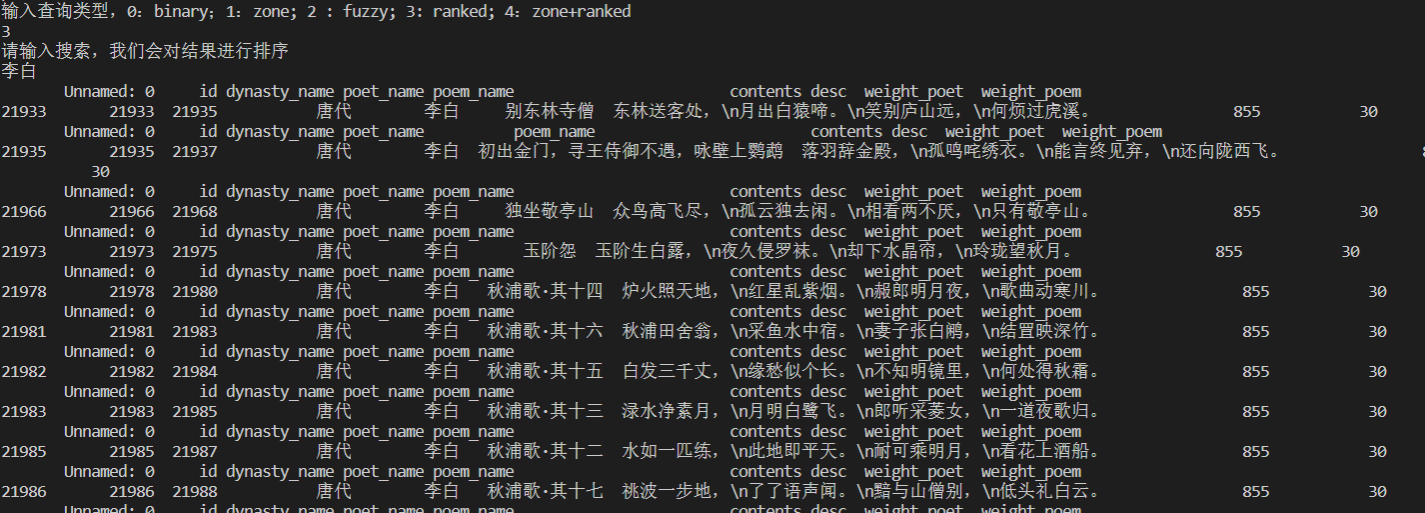
\includegraphics[width=0.8\textwidth]{figure/rank-2.png}
\end{minipage}
}
\caption{Rank Search example: we search '李白' in Boolean Search and in Rank Search, and we can find that, in Boolean Search, The first result is not a poem written by 李白, while for Rank Search, we can get it in the first result.}
\label{search-8}
\end{figure*}
\section{Web Interface} \label{sec:web}
We use the Flask framework to build the web front end. We use the Flask framework to build the web front end. The user first goes to \lstinline{index.html}, then enters query and selects the search method. If the user want to use zone search, go to \lstinline{zone_search.html}, enter query and select the zone to search, as shown in Figure \ref{search-11}. The user's query and selected search method are passed to \lstinline{results.html} through a post request, the search is executed and the output is printed.
\begin{figure*}[h]
\centering
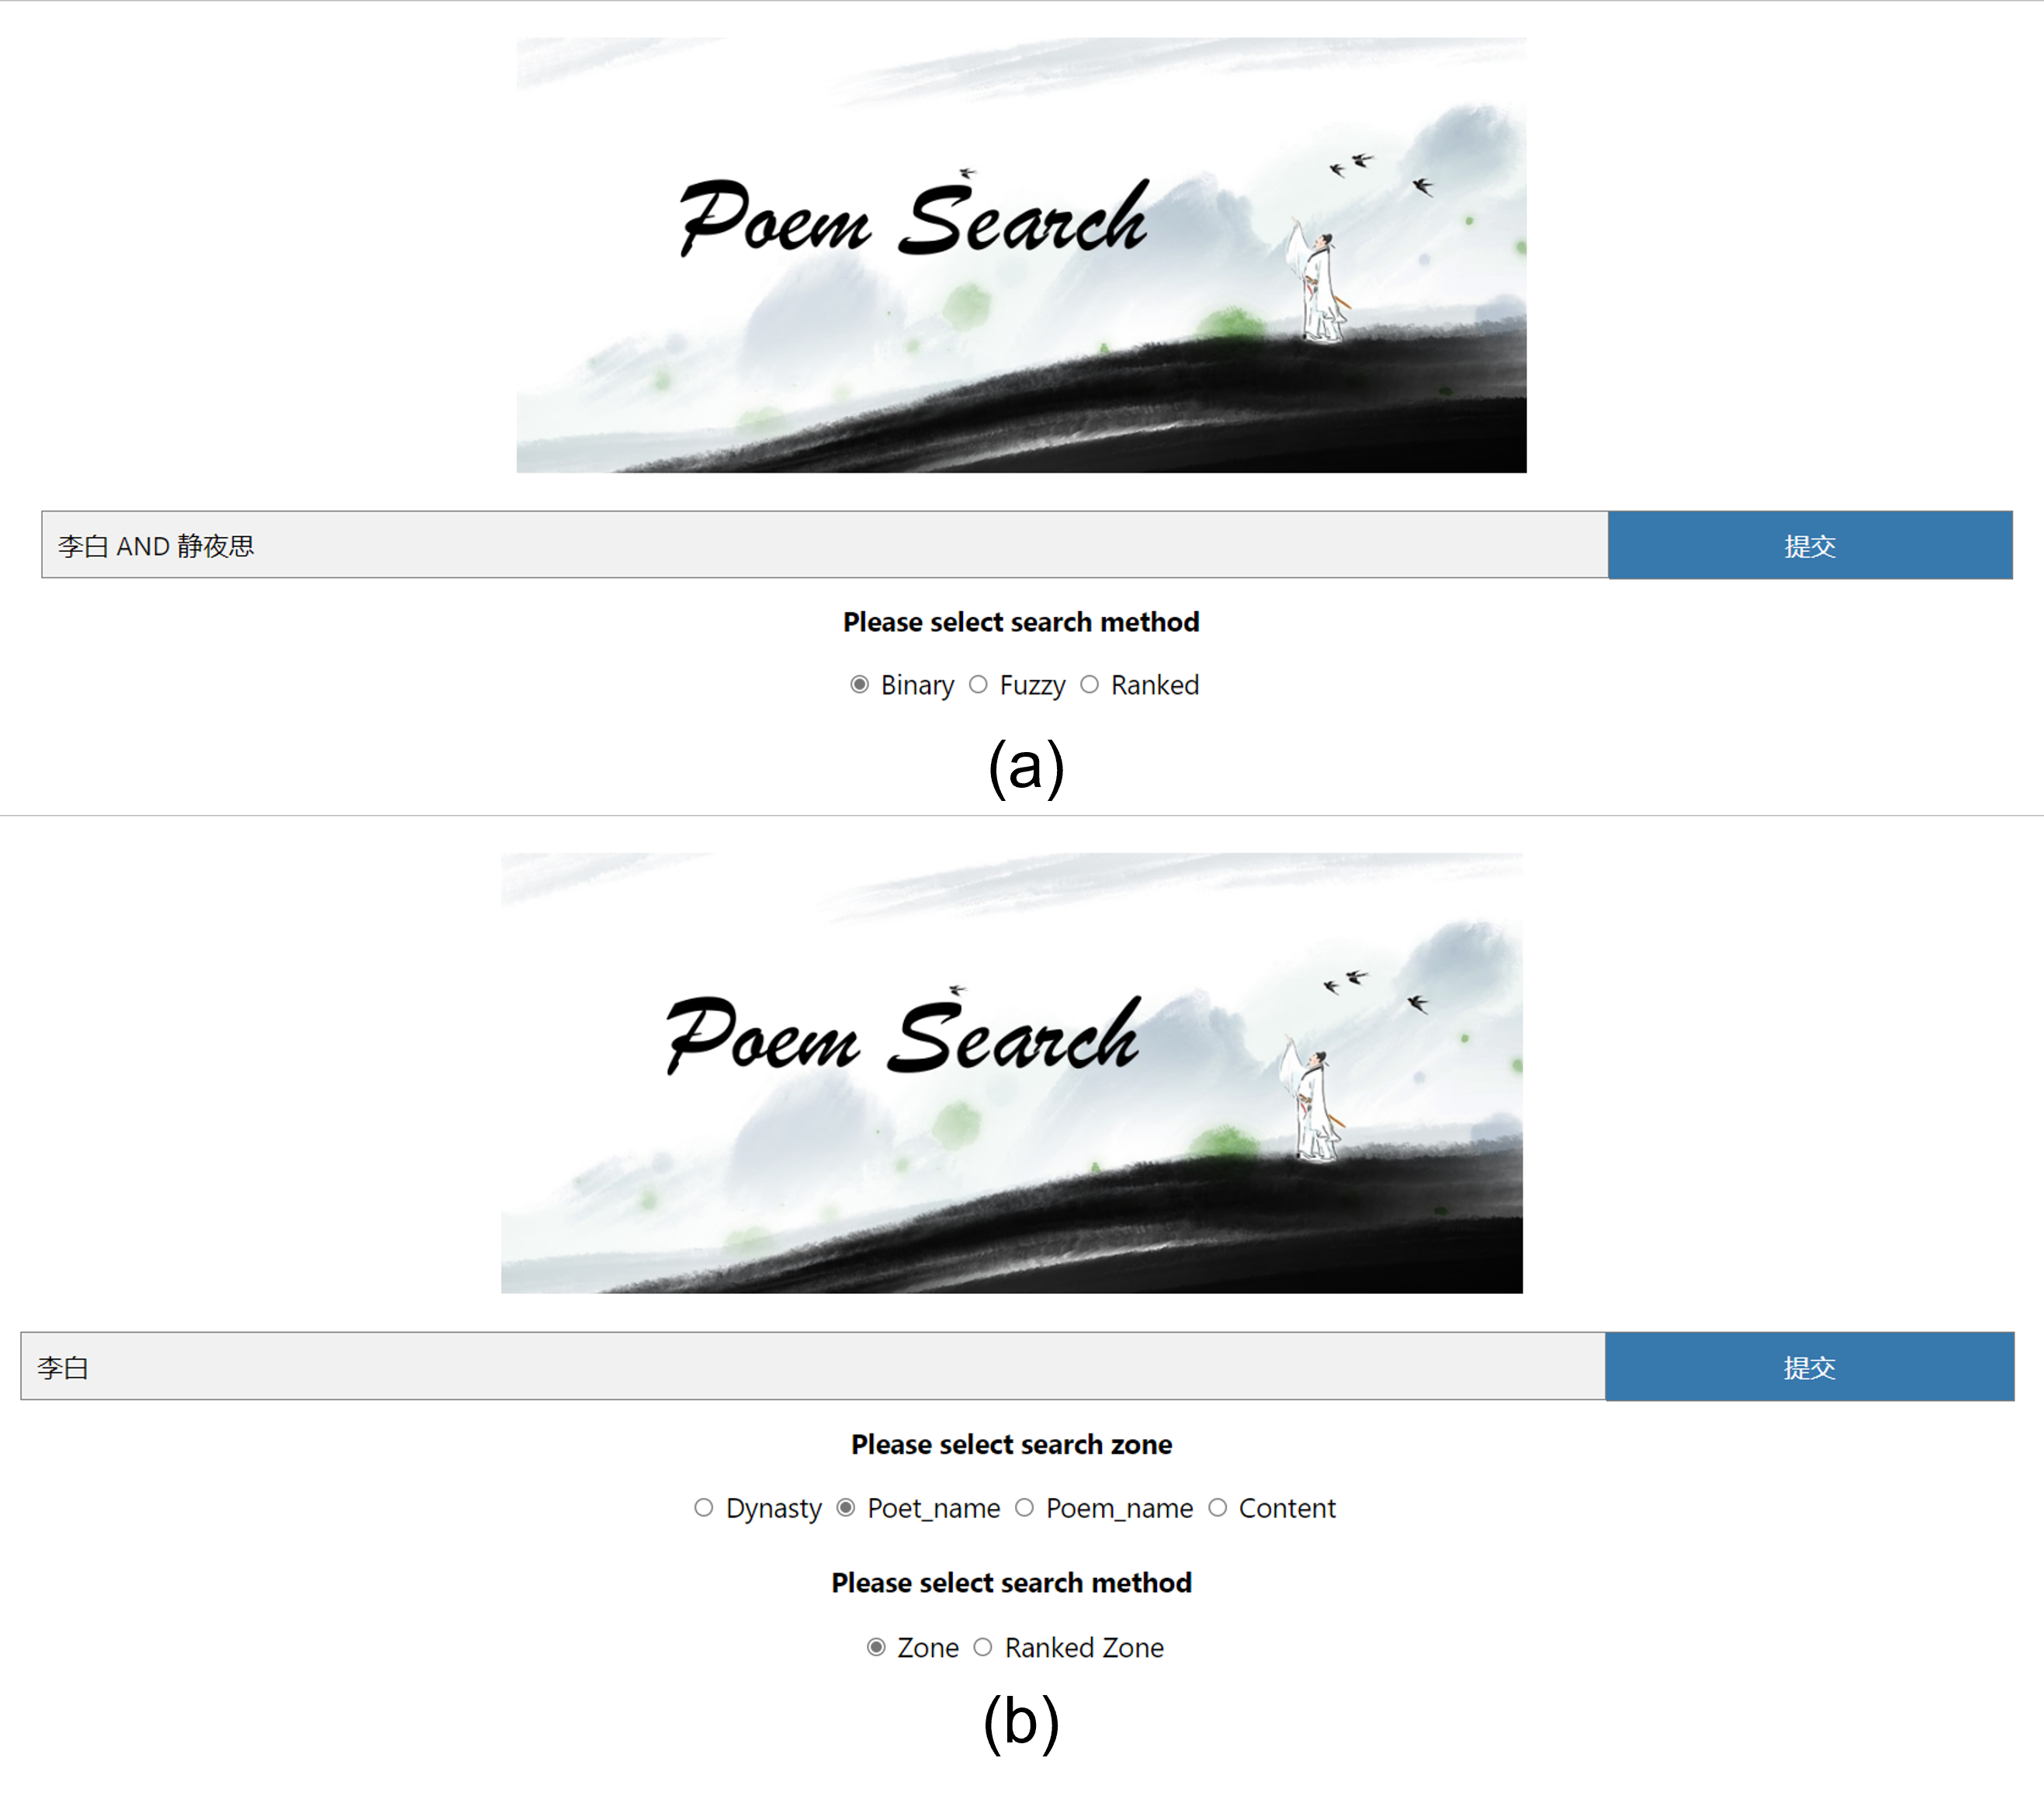
\includegraphics[width=0.7\textwidth]{figure/interface.png}
\caption{(a)\lstinline{index.html} (b)\lstinline{zone_search.html}}
\label{search-11}
\end{figure*}
For binary search, fuzzy search and ranked search, \lstinline{results.html} unpacks the form sent by the user through the request, and selects the corresponding search model to process the query according to the search method. Examples are shown in Figure \ref{search-9}.
\begin{figure*}[h]
\centering
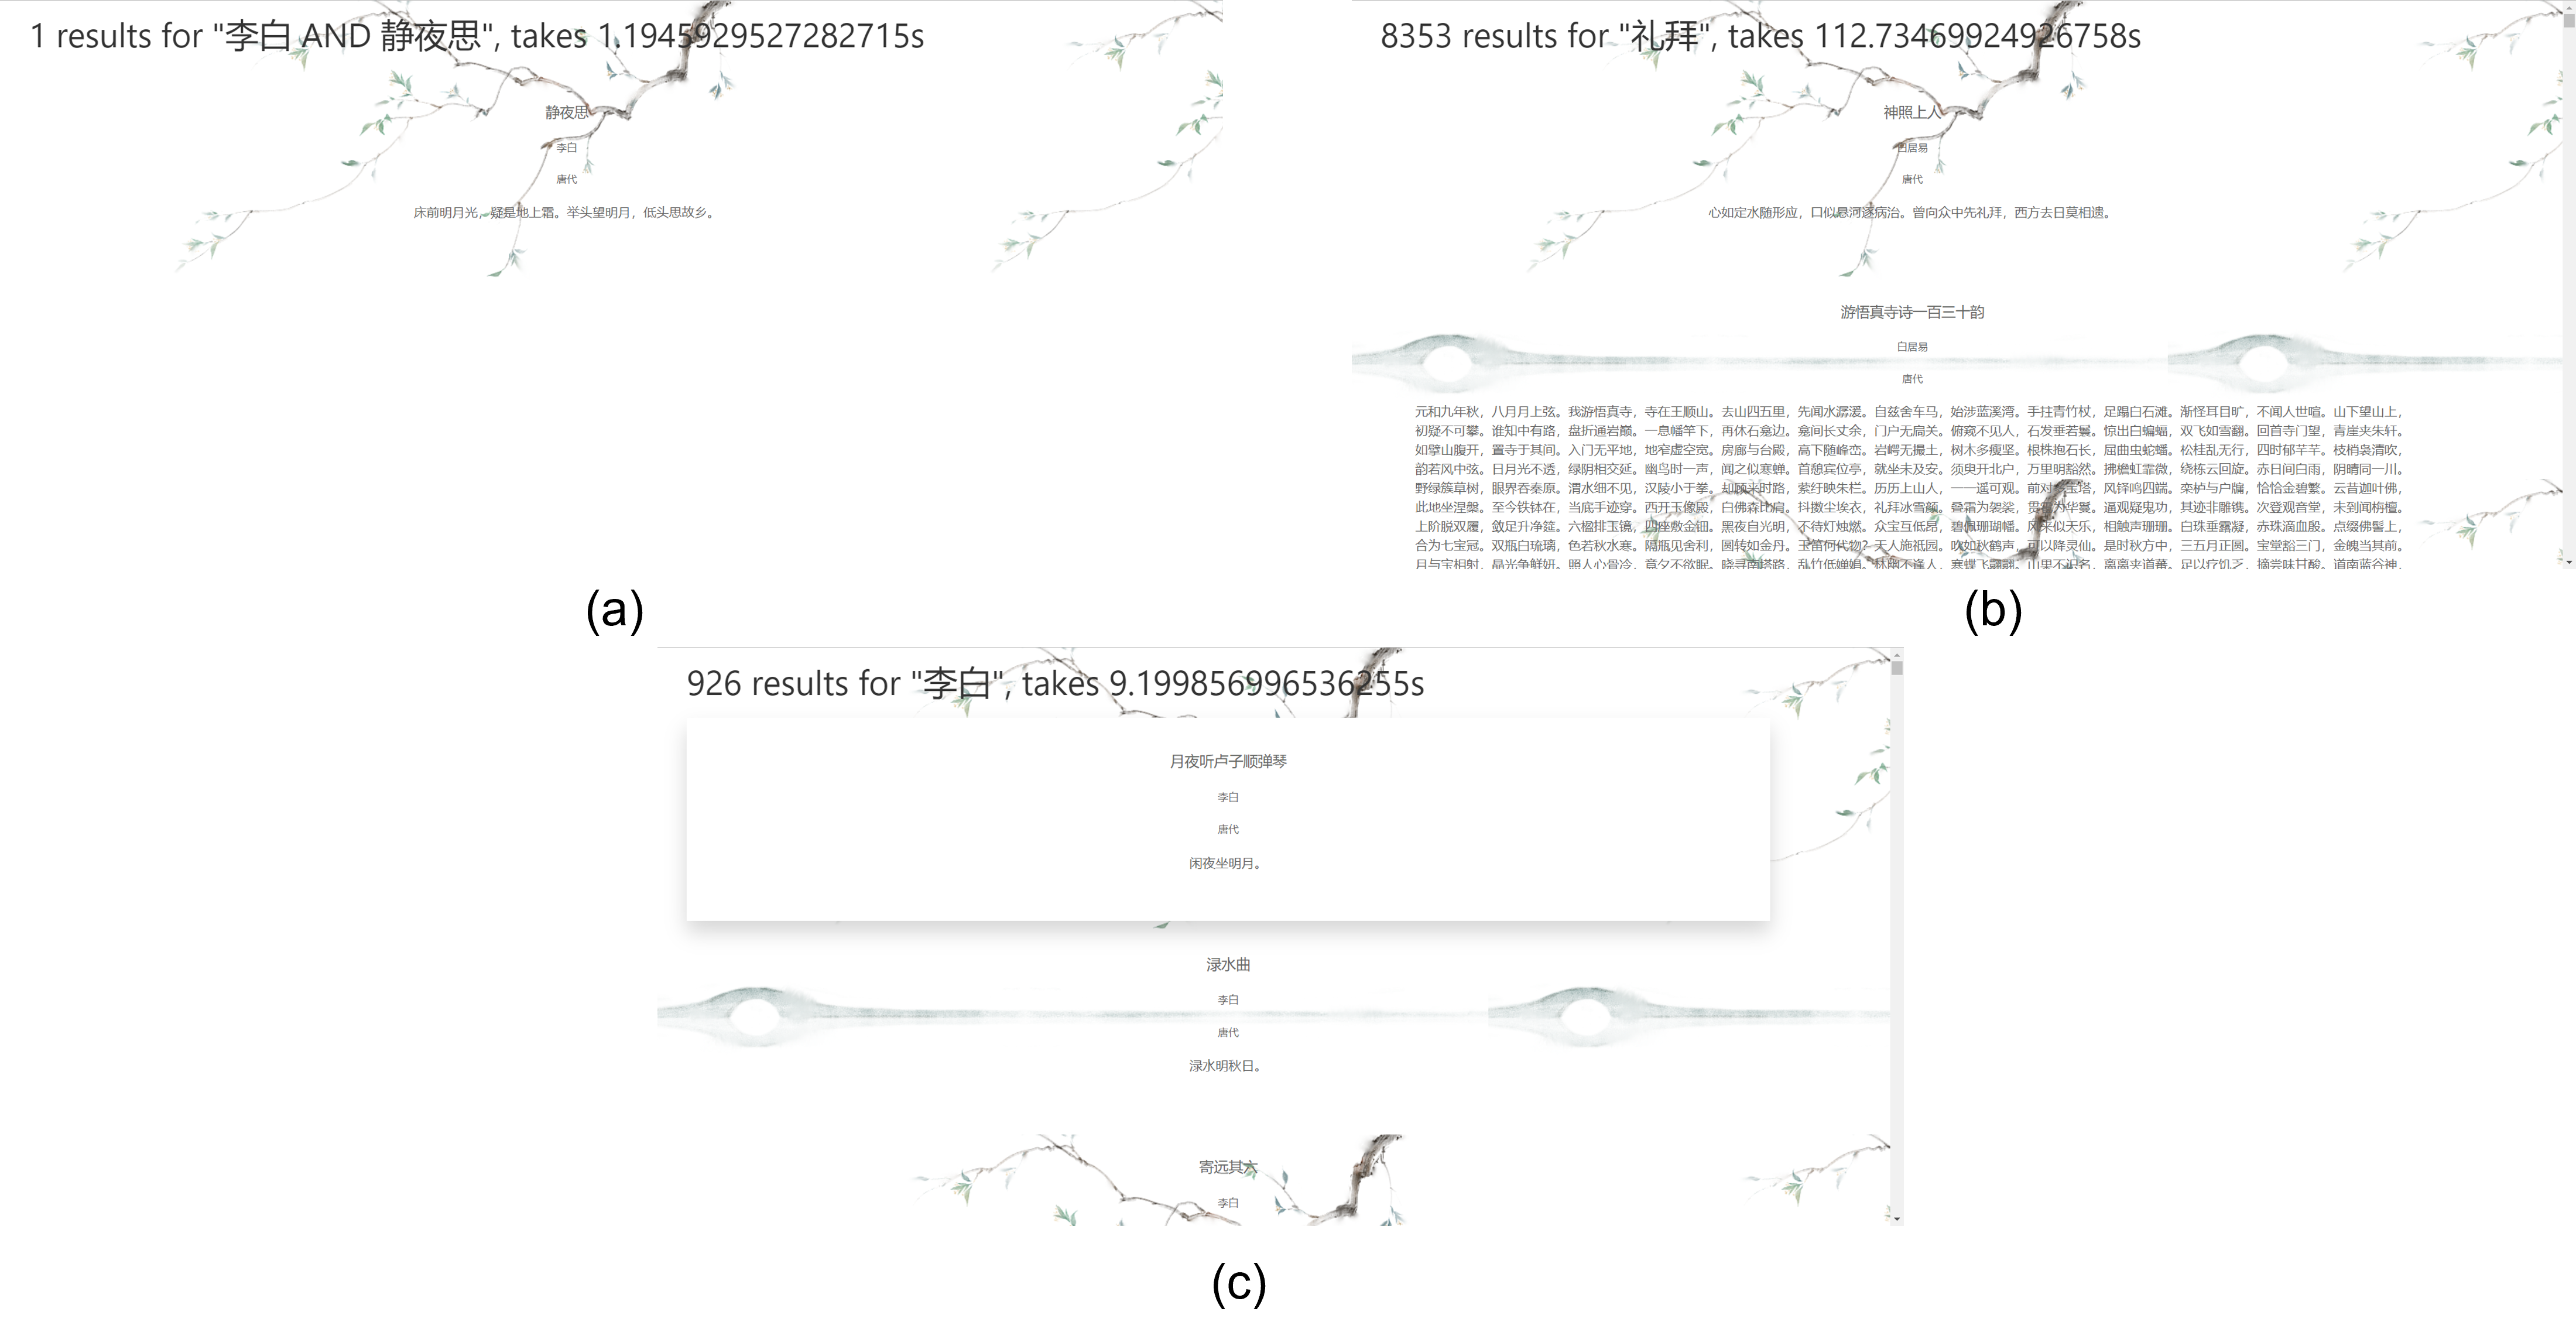
\includegraphics[width=0.7\textwidth]{figure/result1.png}
\caption{(a)\lstinline{Binary search} (b)\lstinline{Fuzzy search}(c)\lstinline{Ranked search}}
\label{search-9}
\end{figure*}

Similarly, for zone search, \lstinline{results.html} unpacks the form sent by the user through the request, selects the zone search search model according to the search method, and processes the query by dynasty, poet, poem name and content according to the corresponding zone, as shown in Figure \ref{search-10}. Show.

\begin{figure*}[h]
\centering
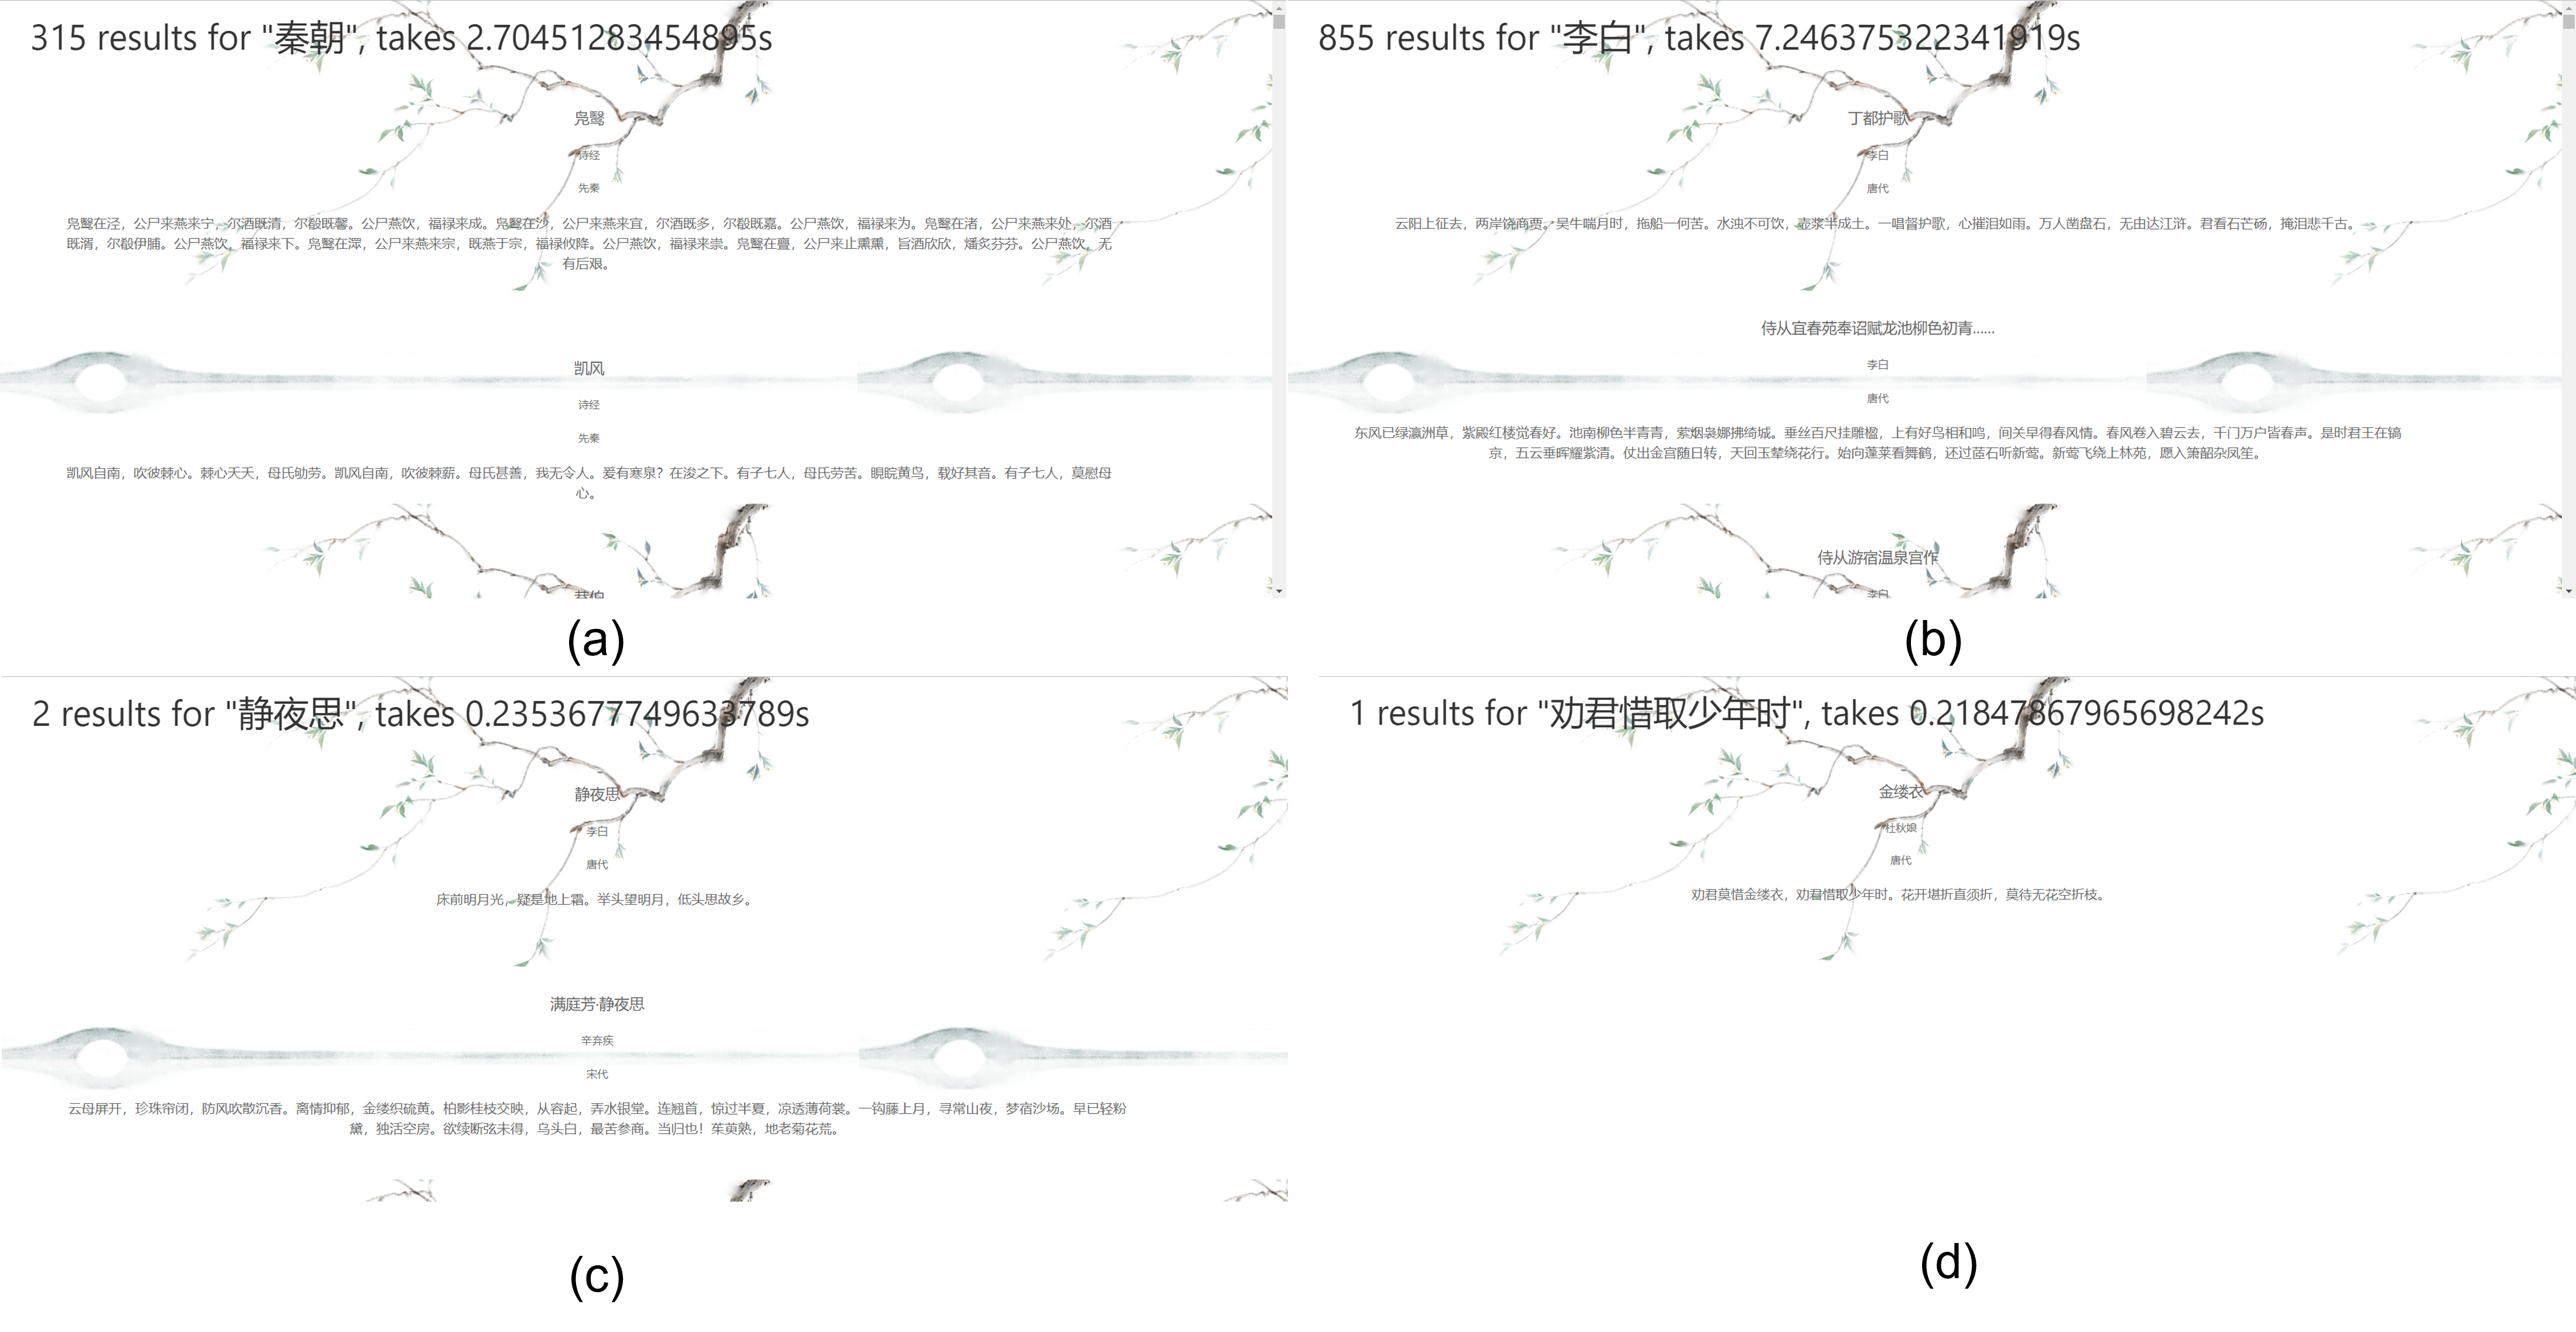
\includegraphics[width=0.7\textwidth]{figure/result2.png}
\caption{(a)\lstinline{zone search for dynasty} (b)\lstinline{zone search for poet}(c)\lstinline{zone search for poem}(d)\lstinline{zone search for content}}
\label{search-10}
\end{figure*}
\section{Thoughts} \label{sec:concl}
During the implementation of this project, we tried many different websites, but due to the continuous development of crawlers and anti-crawlers, many websites have adopted the sweep copy or login to block crawlers. For general considerations, we have chosen this site to crawl. And Scrapy's sophisticated crawler template saves us a lot of time, we only need to do simple processing through the web code to get the data we need. 

While doing pre-processing of the poem names and body, we found some poems with names containing Chinese characters not supported by utf8, so we decisively discarded them. Therefore, we can see that many poems contain vacant parts like * or "$\square$", but of course, this is also partly due to the missing words in the process of circulation. Also, we found that the body of the poems on this site contained an error message like "以上作品共五首", which creates a tremendous amount of work for us.

As for search engine, we can have more improvements for fuzzy search, such as improving the pinyin database to match only the common passwords or misspellings in ancient poems to reduce the search space; on the other hand, we can also convert the final result into pinyin and combine it with the searched pinyin to sort the results. And for rank search, we can manually add a weight to those authors with few works but a strong reputation to get their results further up the list, for example, 张若虚 and 《春江花月夜》。


% As for web, xxxxxxxxxx.

You can see our codes and dataset on the Github \href{https://github.com/yashen32768/Crawl-for-poems}{Crawl-for-poems}.
\bibliography{full_list}

\end{document}